%-----------------------------------------------------------------------------%
\chapter{\babEmpat}
\label{bab:4}

Bab ini menjelaskan detail arsitektur dan implementasi dari aplikasi PeerToCP. Selain itu, terdapat penjelasan singkat serta alasan pemilihan beberapa teknologi, termasuk \textit{library} dan \textit{modul} yang digunakan dalam implementasi, diikuti dengan \textit{usecase} atau fitur sistem. Bab ini juga memaparkan detail skenario pengujian dan metode evaluasi disusun berdasarkan aspek-aspek sistem pada variasi yang akan dibandingkan.

\section{\textit{Library} dan \textit{Framework} Terkait}

Terdapat beberapa modul dan \textit{library} pihak ketiga yang dimanfaatkan dalam pengembangan sistem aplikasi PeerToCP yang dibahas dalam penelitian ini. Berbagai \textit{framework} dan \textit{library} ini merupakan hasil penelitian dan implementasi oleh para pengembang sebelumnya. Pemilihan penggunaan setiap teknologi ini dipertimbangkan dengan alasan tertentu, salah satunya adalah Electron, yang menjadi basis pengembangan aplikasi \textit{desktop} pada PeerToCP.

Electron merupakan salah satu \textit{framework} \textit{desktop} yang sistem kerja pengembangannya serupa dengan komponen web. Bagian tampilan atau \textit{frontend} dari Electron memanfaatkan aplikasi \textit{Chromium} yang dapat mengolah bahasa \textit{markup} web, seperti HTML (\textit{HyperText Markup Language}), CSS (\textit{Cascading Style Sheets}), serta JavaScript. Bagian belakang atau \textit{backend} dari Electron berjalan dengan \textit{environment runtime} Node.js~\citep{kredpattanakul2018transforming, miglanielectron}. Node.js merupakan bahasa yang menggunakan \textit{syntax} yang serupa dengan JavaScript dan dapat dikompilasi melalui kompilator yang disebut V8 engine~\citep{tilkov2010node}.

Salah satu keuntungan menggunakan Electron adalah aplikasinya yang bersifat \textit{cross-platform} atau dapat berjalan di beragam sistem operasi, seperti Windows, GNU/Linux, atau MacOS. Electron mengizinkan akses berbagai macam fungsi antarmuka sistem operasi, seperti memanggil subproses pada sistem dan menulis berkas. Karena \textit{frontend}-nya yang menggunakan bahasa web pula, aplikasi yang dibuat dengan Electron cenderung lebih mudah untuk dipindahkan dan diadaptasi dengan fungsi terbatas pada web. Selain Electron, masih terdapat beberapa alternatif \textit{desktop-based framework} lain seperti Qt yang berbasis C++ dan Tauri yang berbasis Rust. Pemilihan Electron dipilih karena beberapa \textit{library} \textit{operational transformation}, CRDT, WebSocket, dan WebRTC yang umum digunakan sudah tersedia implementasinya dalam JavaScript dan dapat digunakan melalui Node.js.

CodeMirror digunakan dalam komponen editor kode dan berperan sebagai media interaksi pengguna dengan sistem aplikasi pada \textit{frontend}. CodeMirror sendiri disusun untuk dapat di-\textit{render} oleh peramban web dan mengolah teks dengan sistem \textit{state} disertai operasi perubahan yang bersifat modular. CodeMirror menyediakan banyak ekstensi, aksesibilitas tinggi, serta dukungan untuk berbagai macam bahasa pemrograman. CodeMirror pada PeerToCP dimanfaatkan pula terutama sebagai perantara dengan Yjs, sebuah \textit{library} CRDT yang sudah diintegrasikan dengan CodeMirror.

Yjs merupakan sebuah \textit{library} yang mengimplementasi CRDT yang disebut YATA (\textit{Yet Another Transformation Approach})~\citep{Nicolaescu2016yjs}. Yjs terdiri dari beberapa bagian, yaitu YDocs yang merupakan bagian utama implementasi berbagai struktur data untuk CRDT, ada pula YText yang merupakan variasi CRDT untuk operasi-operasi pada teks, serta YMap dan YArray yang dikombinasikan untuk menyimpan \textit{shell} dan riwayatnya. Dalam penelitian ini, digunakan tiga struktur data CRDT tersebut yang abstraksinya berbeda-beda. Yjs juga merupakan \textit{library} yang tidak terpaku pada sebuah arsitektur. Dalam penelitian ini digunakan dua \textit{provider} jaringan yang dapat berintegrasi dengan YDocs, yaitu YWebRTC dan YWebSocket. Kedua provider ini masing-masing mengintegrasikan YDocs dengan jaringan berarsitektur \textit{full-mesh peer-to-peer} serta \textit{client-server} secara berturut-turut. Yjs memiliki banyak pengembang aktif dan hingga kini masih di-\textit{maintain} dan dikembangkan, sehingga \textit{library} Yjs dipilih dalam penelitian ini.

Untuk variasi \textit{operational transformation} dari PeerToCP, penelitian ini memanfaatkan ekstensi \textit{collaborative editing} dari CodeMirror yaitu @codemirror/collab. \textit{Provider} jaringan untuk arsitektur \textit{client-server} yang dikembangkan untuk metode ini menggunakan \textit{library} rpc-websockets yang dimodifikasi sehingga dapat dimanfaatkan untuk melakukan \textit{broadcast}, \textit{specific-messaging} ke klien tertentu, serta fungsionalitas pemanggilan RPC (\textit{Remote-Procedure Call}) berbentuk \textit{promise} secara \textit{asynchronous} dan \textit{non-blocking}.

Pada variasi PeerToCP dengan metode OT, penyimpanan \textit{shell} diimplementasi menggunakan prinsip OT dan sifat \textit{append-only array} untuk menyederhanakan kompleksitas program. Operasi-operasi yang dapat dilakukan pada \textit{shell} ialah berupa \textit{keystroke} masukan pengguna. Secara khusus, beberapa \textit{keystroke} diperlakukan oleh terminal secara harfiah dan program yang berjalan pada \textit{shell} tersebut sendiri yang harus menangani bagaimana \textit{keystroke} tersebut akan diperlakukan. Misalnya, operasi penghapusan atau melakukan \textit{backspace} secara bawaan pada masukan \textit{shell} diartikan sebagai menambahkan tiga karakter ``$\texttt{\char`\\ b \char`\\ b}$'' (tanpa tanda petik) atau ekuivalen dengan memindahkan \textit{cursor} ke kiri, memasukkan karakter \textit{whitespace}, dan memindahkan \textit{cursor} ke kiri kembali. Dalam penelitian ini, aspek kolaborasi dari \textit{shell} memperlakukan setiap klien untuk memberikan \textit{keystroke} pada satu kanal yang sama tanpa \textit{positional cursor} ganda seperti pada editor kode.

Untuk memenuhi komponen penjalanan program pada suatu \textit{shell} yang dapat diakses oleh setiap klien dalam jaringan, dibutuhkan suatu \textit{library} untuk mengakses sistem operasi untuk melakukan kompilasi terhadap kode. Kompilasi merupakan proses mengonversi kode dari bahasa dengan level yang lebih tinggi dan dapat dimengerti oleh manusia menjadi kode biner yang dapat dimengerti oleh mesin~\citep{aho1985compilers}. Pada penelitian ini, selain editor kode yang bersifat kolaboratif, proses kompilasi berkas kode tunggal juga dapat dilakukan oleh setiap pengguna. Proses kompilasi ini membutuhkan kompilator yang terpasang pada suatu sistem operasi. Pada Node.js, salah satu \textit{library} yang dapat digunakan untuk mengaksesnya ialah Node-pty.

Node-pty merupakan \textit{library} Node.js yang menyediakan antarmuka untuk melakukan \textit{fork} proses dengan deskriptor berkas \textit{pseudoterminal}. Node-pty mengizinkan adanya aliran data untuk baca dan tulis dengan proses berjalan pada kernel. Node-pty berguna untuk menjalankan berkas hasil kompilasi yang bersifat CLI (\textit{Command Line Interface}) yang tidak memiliki tampilan grafik untuk pengguna. Node-pty dipilih karena banyak digunakan dan bersifat \textit{cross-platform}. Aplikasi ini juga membutuhkan bagian \textit{frontend} untuk menampilkannya, dan digunakan Xterm.js. \textit{Library} ini merupakan salah satu komponen yang menampilkan terminal pada web. Xterm.js memiliki antarmuka yang bisa menerima dan meneruskan data dari peramban (\textit{browser}) yang dapat dihubungkan dengan sebuah proses berjalan pada sistem. Xterm.js dikembangkan tanpa memerlukan dependensi, sehingga dipilih dalam pengembangan sistem ini.

\section{Desain Sistem}

Aplikasi PeerToCP didesain sebagai sebuah aplikasi \textit{desktop-based}, yang berarti dijalankan secara langsung pada komputer. Pilihan ini dipertimbangkan untuk mempermudah akses secara luring, sehingga tidak dibutuhkan koneksi internet untuk mengakses aplikasi. Selain itu, fitur kompilasi pada suatu \textit{peer} memerlukan akses \textit{system-call} yang tidak disediakan pada API peramban web~\citep{v8, spidermonkey}. Peramban web ditetapkan seperti ini untuk mencegah \textit{script} yang berpotensi menyerang sistem operasi komputer tidak dapat dijalankan secara langsung. Berikut ialah \textit{diagram activity} yang menunjukkan garis besar alur penggunaan aplikasi.

\begin{figure}
    \centering
    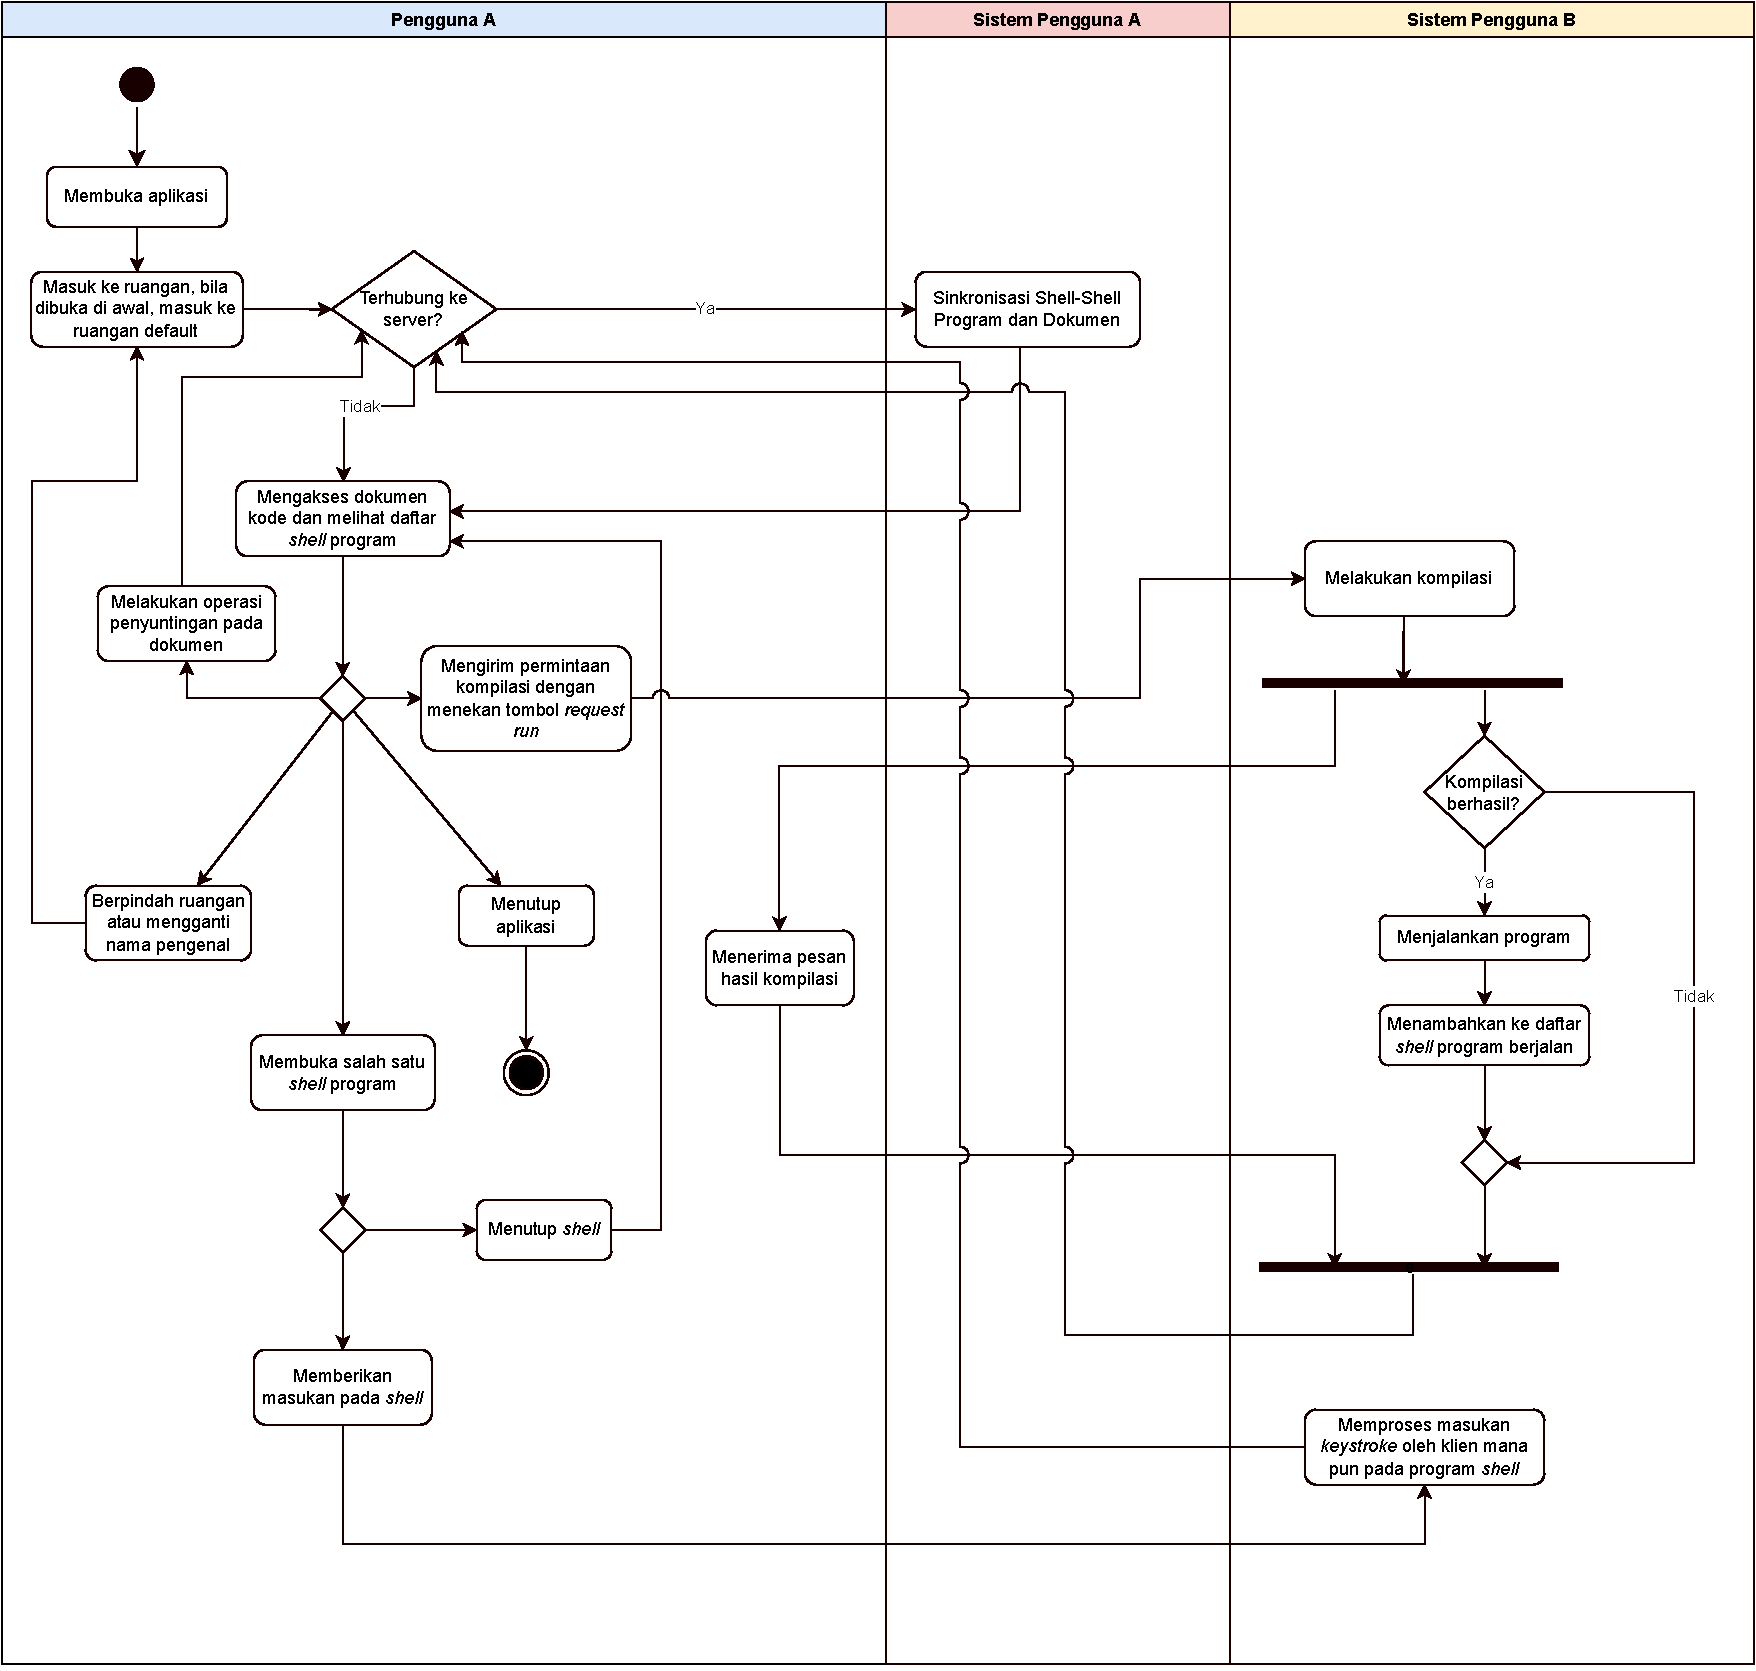
\includegraphics[scale=0.5]{assets/skripsi/Activity_Diagram}
    \caption{\textit{Activity Diagram} Alur Penggunaan Secara \textit{High Level}}
    \label{fig:activity}
\end{figure}

Saat pengguna membuka aplikasi, pengguna akan diarahkan untuk masuk ke ruangan awal secara \textit{default}. Pengguna dapat melakukan operasi-operasi penyuntingan pada dokumen dan sinkronisasi dilakukan secara terus-menerus dengan \textit{publish-subscribe design pattern} sehingga memberikan respons tanpa perlu mengecek atau \textit{polling} saat terjadi \textit{update} yang terjadi antarpengguna. \textit{Request} atau permintaan kompilasi dapat diajukan kepada pengguna mana pun pada sebuah jaringan, termasuk permintaan kepada pengguna tersebut sendiri. Aplikasi PeerToCP akan mencoba mengirimkan pesan kepada pengguna yang ditentukan tanpa intervesi dari pengguna lain dalam jaringan. Apabila permintaan berhasil diterima, sistem pada penerima permintaan akan melakukan proses kompilasi dan memasukkan \textit{shell} program berjalan dengan ID tertentu ke daftar \textit{shell} yang dapat diakses oleh setiap klien dalam jaringan. Daftar \textit{shell} dan kontennya ini disimpan dalam bentuk \textit{object} pada \textit{JavaScript}.

Pada gambar~\ref{fig:activity}, perilaku sinkronisasi \textit{shell}-\textit{shell} pada program dan dokumen dilakukan bergantung dengan variasi implementasi dari program. Pada arsitektur \textit{client-server}, sistem aplikasi pengguna A akan berhubungan dan melakukan sinkronisasi dengan server. Sementara pada arsitektur \textit{peer-to-peer}, sistem aplikasi pengguna A akan berhubungan langsung dan melakukan sinkronisasi dengan \textit{peer} lain. Selain itu, permintaan dan transmisi pesan hasil kompilasi dilakukan melalui pengiriman pesan secara langsung pada arsitektur \textit{peer-to-peer}, namun harus melalui perantara server pada arsitektur \textit{client-server}.

\section{CRDT (\textit{Conflict-Free Replicated Data Type}) Berbasis \textit{Peer-To-Peer} dan \textit{Client-Server}}
\label{sec:desain_crdt}

CRDT pada dua skenario arsitektur dalam penelitian ini menggunakan library CRDT Yjs. Setiap \textit{peer} atau klien memiliki replika yang direpresentasikan dalam tipe data YDocs. YDocs dapat terdiri dari beberapa CRDT \textit{nested} untuk menyimpan data-datanya, dalam penelitian ini \textit{shell} direpresentasikan sebagai sebuah CRDT YMap yang memetakan \textit{id} sebuah \textit{shell} ke sebuah CRDT YArray yang berisi kontennya. Implementasi dari variasi \textit{peer-to-peer} menggunakan \textit{library} penyedia jaringan YWebRTC yang telah dimodifikasi dengan antarmuka untuk mengirim pesan ke \textit{peer} tertentu melalui jaringan RTCDataChannel. \textit{Keystroke} yang diberikan oleh sebuah \textit{peer} tertentu akan dikirim langsung pada \textit{peer host} yang menjalankan programnya, kemudian \textit{peer host} akan menambahkan hasil \textit{keystroke} pada struktur \textit{array} yang berkorespondensi dengan \textit{shell} yang berisi program tersebut.

\begin{figure}
    \centering
    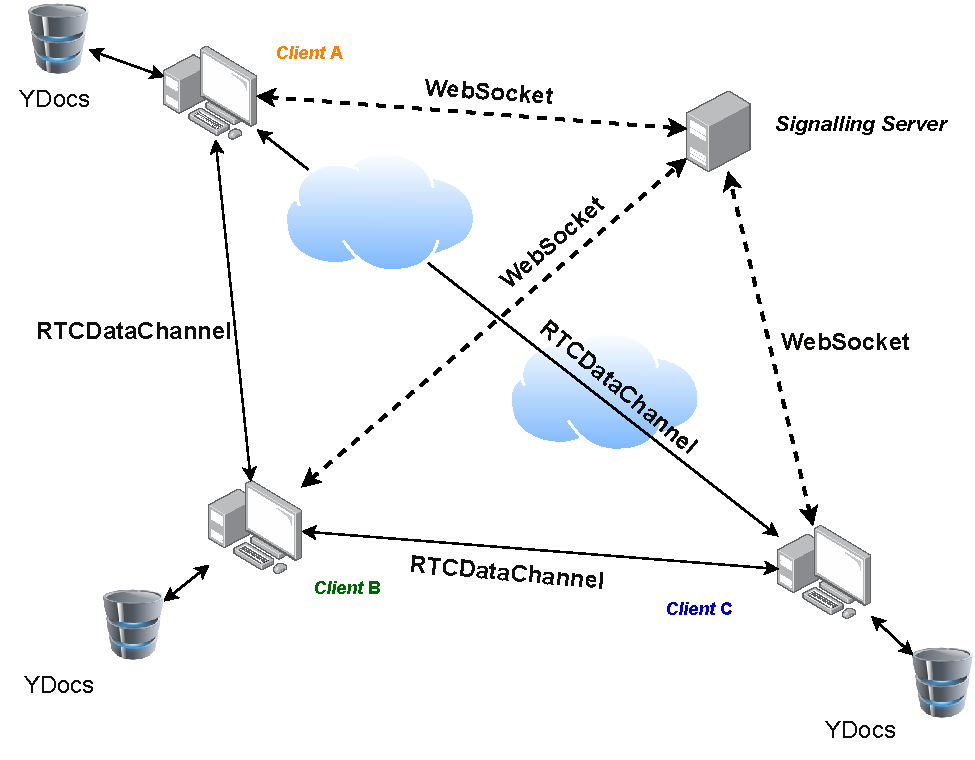
\includegraphics[scale=0.65]{assets/skripsi/Arsitektur_WebRTC_CRDT}
    \caption{Arsitektur yang Menggunakan WebRTC dengan WebSocket \textit{Signalling} dan CRDT}
\end{figure}

\begin{figure}
    \centering
    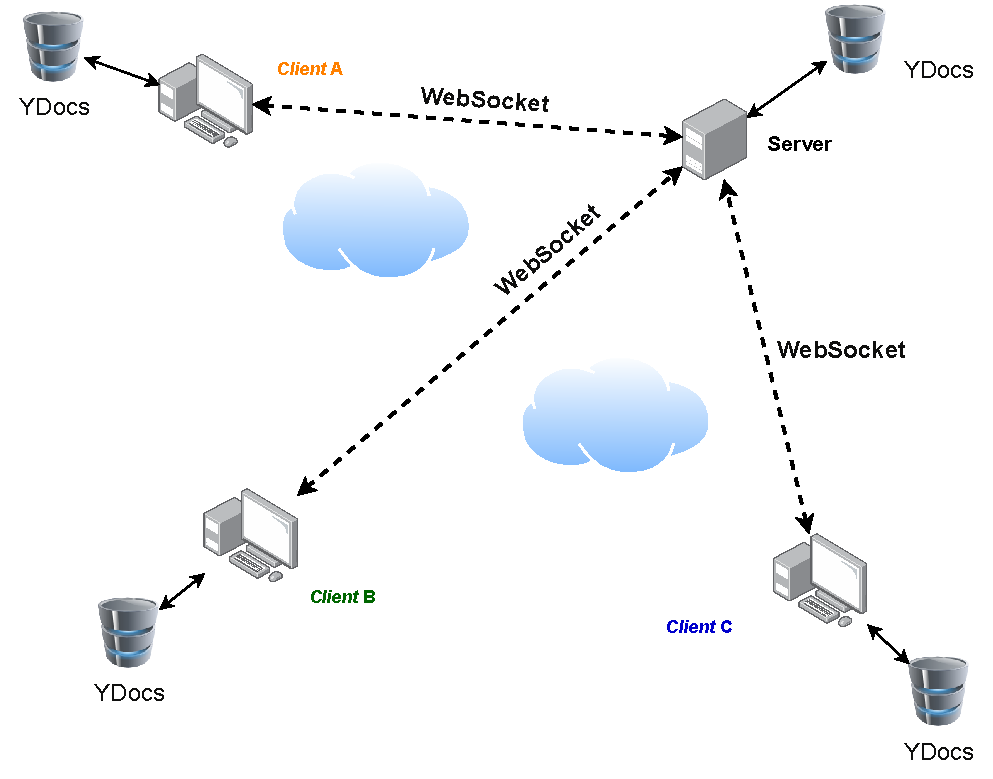
\includegraphics[scale=0.65]{assets/skripsi/Arsitektur_WebSocket_CRDT}
    \caption{Arsitektur yang Menggunakan WebSocket dan \textit{CRDT}}
\end{figure}

Perbedaan antara kedua implementasi arsitektur CRDT ini terdapat pada \textit{provider} atau penyedia jaringannya. Pada arsitektur \textit{client-server}, penelitian ini menggunakan \textit{library} YWebSocket yang telah dimodifikasi pula untuk dapat mengirim pesan kepada klien tertentu dalam sebuah jaringan melalui server. Penyedia jaringan pada dasarnya memberikan abstraksi bagi setiap \textit{peer} atau klien dalam sebuah jaringan terdistribusi untuk berhubungan satu sama lain. Terdapat fitur tambahan bagi server pada arsitektur ini untuk dapat melakukan persistensi data. Persistensi ini mengizinkan untuk server menyimpan salah satu replika dari dokumen, sehingga dokumen masih akan tetap ada walaupun tidak ada klien yang terhubung. Selain pada CRDT, arsitektur \textit{client-server} digunakan pada metode \textit{operational transformation} untuk menjaga kesamaan replika dalam suatu jaringan sistem terdistribusi. Variasi PeerToCP dengan \textit{operational transformation} yang hanya memenuhi \textit{Transformation Property 1} berbasis \textit{client-server} menjadi salah satu variasi yang dibandingkan dalam penelitian ini.

\section{Metode \textit{Operational Transformation} Berbasis \textit{Client-Server}}
\label{sec:design_ot}

Untuk suatu dokumen yang hanya menyimpan teks biasa, operasi \textit{operational transformation} yang hanya memenuhi sifat \textit{TP1} dapat diimplementasi dengan sederhana dalam arsitektur \textit{client-server}. Aplikasi PeerToCP dengan variasi ini menggunakan \textit{library} @codemirror/colab yang mengimplementasikan \textit{operational transformation} yang menyimpan operasi perubahan CodeMirror dalam bentuk \textit{delta}. Algoritma bekerja dengan menyimpan sebuah \textit{array} perubahan lokal yang belum diketahui oleh server. Perubahan-perubahan lokal beserta versi dokumen terbaru dari server yang sudah diaplikasikan di lokal akan dikirimkan secara berkala dengan mekanisme RPC \textit{over} WebSocket. Mekanisme RPC \textit{over} WebSocket pada dasarnya mengizinkan alur \textit{non-blocking} dalam menunggu balasan sebelum mengirimkan percobaan pengiriman perubahan lainnya. Apabila versi dasar dari server lebih baru daripada versi lokal, maka pengiriman perubahan akan ditolak, dan server akan memberikan respons kepada klien tersebut untuk melakukan \textit{rebase} atau menambahkan \textit{update} yang terdapat di server terlebih dahulu sebelum dapat mengirim percobaan pengiriman kembali.

\begin{figure}
    \centering
    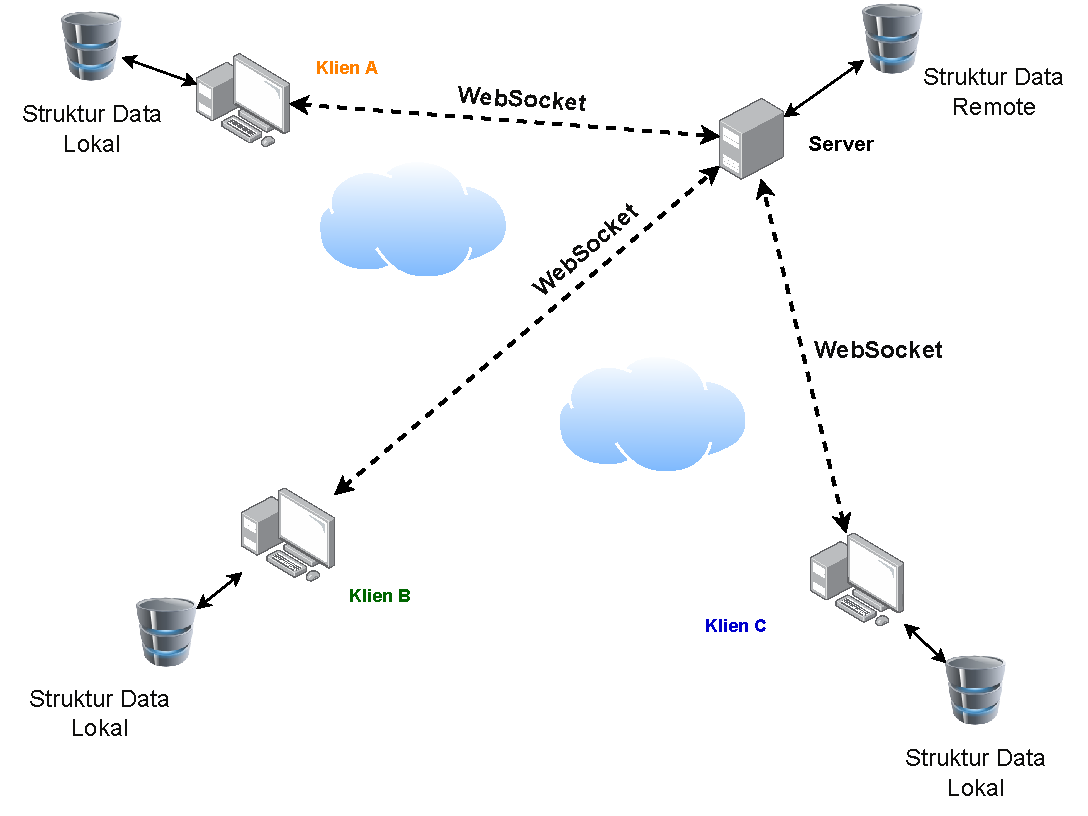
\includegraphics[scale=0.65]{assets/skripsi/Arsitektur_WebSocket_OT}
    \caption{Arsitektur yang Menggunakan WebSocket dan \textit{Operational Transformation}}
    \label{fig:websocket_ot}
\end{figure}

Perubahan \textit{remote} yang diterima dari server akan ditransformasikan satu sama lain dengan perubahan lokal yang belum diketahui oleh server. Perubahan lokal kemudian akan ditimpa dengan perubahan yang sudah ditransformasikan dengan perubahan \textit{remote}. Percobaan pengiriman yang dikirim selanjutnya akan mengikuti perubahan yang sudah ditransformasikan ini. \textit{Operational transformation} hanya terjadi di lokal dan perubahan akan diperbarui secara berurutan, sehingga setiap dokumen dalam jaringan memiliki replika yang berujung identik dan konvergen.

Hal yang serupa diterapkan pula untuk \textit{shell} program yang berjalan. Saat suatu klien memberikan \textit{keystroke} pada salah satu \textit{shell} yang aktif, \textit{keystroke} akan dikirimkan melalui mekanisme yang serupa, namun akan diarahkan ke klien yang menjadi \textit{host} atau menjalankan programnya. Selanjutnya, perubahan \textit{shell} akan dikirimkan berkala pada server selama ada perubahan yang belum diterima atau diketahui server. Saat terjadi perubahan, server akan melakukan pengumuman kepada setiap klien untuk melakukan \textit{pull}. Karena respons \textit{shell} bergantung pada klien \textit{host}, maka pembaharuan tidak perlu diterapkan fungsi transformasi seperti pada OT teks biasa. Salah satu aspek lainnya ialah \textit{position mapping} yang tidak perlu ditangani karena kursor akan selalu berada di sebelah kanan karakter terakhir. Operasi seperti mekanisme \textit{update} yang dilaksanakan secara serial ini diterapkan untuk mencegah terjadinya \textit{race condition} pada saat gangguan jaringan.

Beragam arsitektur yang sudah dipaparkan pada subbab-subbab sebelummya merupakan bagian \textit{backend} dari suatu antarmuka editor yang sama, sehingga penilaian secara \textit{end-to-end} yang akan dirasakan oleh pengguna menjadi tolok ukur yang logis dalam penelitian ini. Tolok ukur ini terdiri dari kasus yang mempertimbangkan aspek-aspek yang hendak diuji. Evaluasi dilakukan dengan perlakuan kontrol yang diusahakan identik untuk dapat memberikan hasil yang akurat.

\section{Desain Evaluasi}
\label{sec:desain_evaluasi}

Evaluasi sistem dilakukan dengan layanan Compute Engine Google Cloud Platform. Setiap variasi memiliki server yang di-\textit{deploy} pada \textit{instance} dengan zona daerah \texttt{asia-southeast1-b}, menggunakan mesin bertipe \texttt{e2-medium} yang memiliki 2 vCPUs dan memori RAM 4GiB, serta sistem operasi Debian 11. Alasan dipilihnya mesin dengan tipe ini adalah untuk menghindari proses \textit{benchmarking} atau tolok ukur yang dibatasi oleh spesifikasi sistem. Dalam penelitian ini, \textit{relay server} tidak disediakan untuk \textit{peer} yang tidak dapat terhubung satu sama lain dalam sebuah jaringan \textit{peer-to-peer} berbasis WebRTC. Penelitian ini mengasumsikan inisialisasi koneksi \textit{peer-to-peer} WebRTC selalu berhasil pada variasi ini.

Untuk \textit{instance virtual machine} yang mewakili pengguna, digunakan mesin bertipe \texttt{e2-small} yang memiliki 2 vCPUs, memori Ram 2GiB, dan sistem operasi Debian 11 pula. Mesin pengguna akan di-\textit{deploy} pada \textit{zone} \texttt{asia-southeast2-a}. Setiap mesin pengguna diletakkan pada \textit{zone} yang sama, dan dekat dekat dengan server dengan tujuan untuk mensimulasikan perkiraan penggunaan aplikasi PeerToCP di dunia nyata. Terdapat empat skenario uji yang akan dilakukan terhadap sistem aplikasi. Skenario pertama secara praktis menyimulasikan serangkaian operasi-operasi tertentu terhadap editor teks dengan jumlah \textit{peer} sebanyak $n$ yang berbeda-beda. Jumlah klien atau \textit{peer} yang berbeda bertujuan untuk mewakilkan aspek \textit{scalability}. Terdapat tiga macam operasi acak yang dilakukan sebanyak sepuluh operasi per detik dalam periode uji tiga menit, yaitu:

\begin{enumerate}[nolistsep]
    \item memasukkan (\texttt{insert}) suatu \textit{string} karakter ASCII acak dengan panjang antara 2 hingga 5 secara inklusif;
    \item menghapus (\texttt{delete}) suatu \textit{range} dengan panjang antara 1 hingga 3 secara inklusif;
    \item menimpa (\texttt{replace}) suatu \textit{range} dengan panjang antara 2 hingga 5 dengan \textit{string} karakter ASCII acak dengan jangkauan yang sama.
\end{enumerate}

Operasi-operasi tersebut memiliki rata-rata penambahan sebanyak 15 karakter per detik dan perubahan sebanyak 41.67 karakter per detik (termasuk penghapusan) pada setiap kliennya. Tes dimulai bersamaan menggunakan \textit{timer} bawaan sistem operasi yang secara \textit{default} sudah disinkronisasi. Galat atau \textit{error} yang terdapat pada sinkronisasi waktu \textit{timer} tentunya tidak dapat dihindari, sehingga dianggap tidak ada. Namun, penelitian ini akan menggunakan \textit{instance} yang sama untuk setiap \textit{peer} atau kliennya sehingga mengurangi bias perbedaan \textit{timer} pada setiap klien dalam jaringan. Selain itu, akan ada operasi pemutusan jaringan (\texttt{disconnect}) yang akan terjadi secara acak selama 30 detik di antara satu menit setelah uji skenario dimulai hingga satu menit sebelum uji skenario berakhir. Keadaan akhir editor teks setelah selesai akan sehendaknya terhubung ke server untuk melakukan sinkronisasi terakhir dengan \textit{peer-peer} lain dari server. Selama editor teks tidak terhubung, operasi-operasi lain seperti \texttt{insert}, \texttt{delete}, dan \texttt{replace} masih berjalan pada editor guna menggambarkan aspek \textit{local-first}.

Skenario pertama disusun selayaknya \textit{stress-testing} terhadap operasi-operasi editor teks yang dapat terjadi di dunia nyata. Di akhir tes, sistem menunggu selama satu menit untuk memberikan kelonggaran sinkronisasi. Waktu terakhir \textit{update} atau sinkronisasi akan disimpan untuk dibandingkan pada aspek \textit{responsiveness} dan \textit{scalability}. Nilai cacahan atau \textit{hash} dari dokumen setelah uji skenario juga turut dicatat pada setiap klien atau \textit{peer} serta dibandingkan satu sama lain untuk memenuhi aspek \textit{correctness}. Selain itu, aktivitas RAM, CPU, dan transmisi data dalam jaringan pada setiap klien beserta server akan direkam menggunakan \textit{framework} NetData untuk memenuhi aspek \textit{lightweight} dan \textit{scalability} pula.

Skenario kedua menggunakan \textit{environment} sama dengan skenario sebelumnya. Skenario ini disusun untuk menguji \textit{shell} pada setiap $n$ klien berbeda, yaitu dengan menjalankan suatu program C++ yang akan mencetak 100 bilangan tak bertanda (unsigned) 64-bit acak dengan jeda acak setiap bilangannya selama 500 hingga 1500 milidetik. Selama itu, akan dilakukan operasi pemutusan jaringan pula(\textit{disconnect}) yang akan terjadi secara acak selama 20 detik setelah 10 hingga 40 detik setelah program berjalan. Seperti skenario sebelumnya, waktu sinkronisasi terakhir, aktivitas perangkat, dan nilai cacahan dari setiap \textit{shell} pada setiap klien akan dicatat dan dibandingkan untuk memastikan bahwa setiap pengguna memiliki replika \textit{shell} yang sama.

Skenario ketiga dan terakhir berpusat untuk mengukur latensi dari editor teks dan \textit{shell}. Pada skenario ketiga, $n$ peer disusun serupa dengan dua skenario sebelumnya. Terdapat dua operasi yang akan dilakukan, yaitu memasukkan (\texttt{insert}) \textit{timestamp} pada editor teks dan menimpa (\texttt{replace}) suatu \textit{range} dengan panjang antara 10 hingga 15 karakter dengan \textit{timestamp}. Setiap operasi yang dilakukan memiliki jeda acak selama 500 hingga 1000 milidetik guna menghindari operasi yang dilakukan secara bersamaan dalam periode yang tetap. Setiap klien atau \textit{peer} kemudian menangkap \textit{timestamp} dan mengukur latensi perbedaan saat \textit{timestamp} dicetak dan \textit{timestamp} diterima pada klien lainnya. Pada skenario keempat, setiap klien akan menjalankan program C++ yang akan mencetak 100 \textit{timestamp} dengan jeda acak selama 500 hingga 1500 milidetik. Setiap klien kemudian menangkap setiap \textit{event} ini dan mengukur latensinya dengan cara serupa, yaitu dengan menghitung selisih pemasukan konten timestamp oleh sebuah \textit{shell host} (pengguna yang menjalankan program) dengan penerimaan pada setiap pengguna lainnya. Pada skenario ketiga dan keempat ini, tidak ada operasi pemutusan pengguna dengan tujuan menghasilkan data yang akan dievaluasi pada aspek \textit{responsiveness} yang lebih akurat.